\section{Электрический диполь}

	Пусть сумма всех зарядов\index{Заряд} в~системе\index{Система} равна нулю:
		$$\sum q_i = 0.$$
	Тогда сумма всех положительных зарядов по~модулю равна сумме всех отрицательных зарядов:
		$$\sum_{(+)} q_i = +q, \quad \sum_{(-)} q_i = -q.$$
	Рассмотрим центр заряда\index{Центр!заряда} (аналог центра масс)\index{Центр!масс} (рис.~\ref{fig:dipole1}):
		$$\vec{R}_{(+)}=\frac{\sum_{(+)} q_i\vec{r}_i}{\sum_{(+)} q_i}, \quad \vec{R}_{(-)}=\frac{\sum_{(-)} q_i\vec{r}_i}{\sum_{(-)} q_i}.$$
	\begin{figure}[h!]
		\label{fig:dipole1}
		\centering
		\documentclass{article}

\usepackage[latin1]{inputenc}
\usepackage{pgfplots}
\usepackage{tikz}

\pgfplotsset{compat=1.10}

\begin{document}
\pagestyle{empty}

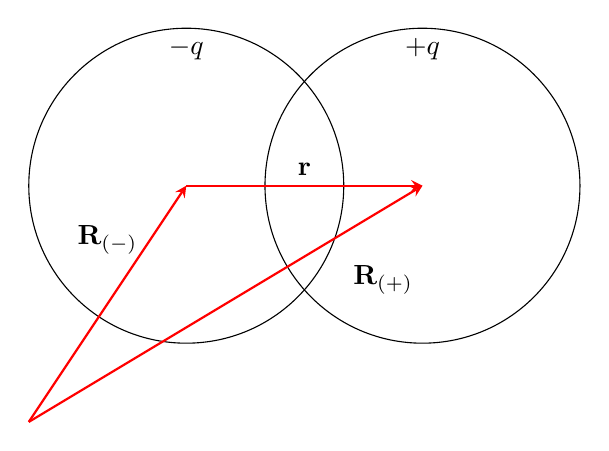
\begin{tikzpicture}[>=stealth]
	\draw[thin] (0, 0) circle [radius=2];
	\draw[thin] (3, 0) circle [radius=2];

	\draw[-latex, red, thick, ->] (0, 0) -- (3, 0);
	\node[above] at (1.5, 0) {$\textbf{r}$};

	\draw[-latex, red, thick, ->] (-2, -3) -- (0, 0);
	\node[above] at (-1, -1) {$\textbf{R}_{(-)}$};

	\draw[-latex, red, thick, ->] (-2, -3) -- (3, 0);
	\node[above] at (2.5, -1.5) {$\textbf{R}_{(+)}$};

	\node[below] at (0, 2) {$-q$};
	\node[below] at (3, 2) {$+q$};
\end{tikzpicture}


\end{document}
		\caption{Электрический диполь}
	\end{figure}
	Полезная характеристика диполя -- дипольный момент\index{Момент!дипольный}:
	\begin{equation}
		\vec{d}=q\vec{r}.
	\end{equation}
	\begin{equation}
		\vec{d}=q(\vec{R}_{(+)}-\vec{R}_{(-)})=\sum_{(+)} q_i\vec{r}_i + \sum_{(-)} q_k\vec{r}_k=\sum_{\text{по всем}} q_i\vec{r}_i.
	\end{equation}
	Рассмотрим диполь во~внешнем постоянном электрическом поле\index{Поле!постоянное}\index{Поле!электрическое}.
	\begin{figure}[h!]
		\label{fig:dipole2}
		\centering
		\documentclass{article}

\usepackage[latin1]{inputenc}
\usepackage{pgfplots}
\usepackage{tikz}
\usetikzlibrary{arrows}

\pgfplotsset{compat=1.10}

\begin{document}
\pagestyle{empty}

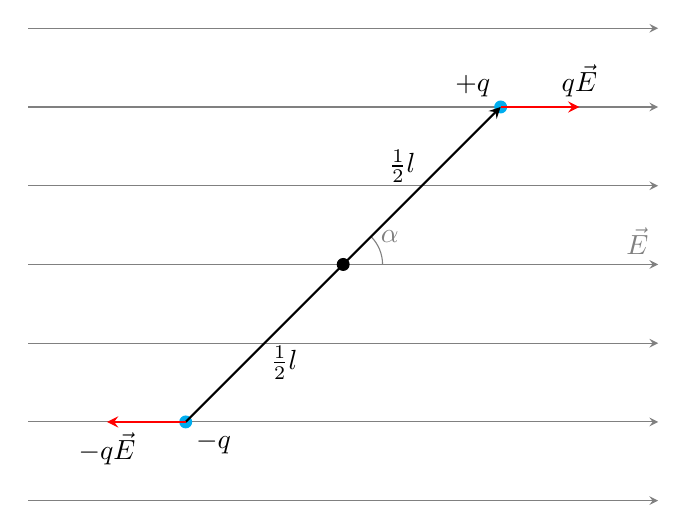
\begin{tikzpicture}[>=stealth]
	\foreach \y in {-3,-2,...,3}
		\draw[-latex, thin, gray, ->] (-4, \y) -- (4, \y);
	\node[gray, above left] at (4, 0) {$\vec{E}$};

	\draw[fill] (0, 0) circle [radius=0.075];
	\draw[cyan, fill] (2, 2) circle [radius=0.075];
	\draw[cyan, fill] (-2, -2) circle [radius=0.075];

	\node at (0.75, 1.25) {$\frac{1}{2}l$};
	\node at (-0.75, -1.25) {$\frac{1}{2}l$};

	\draw[gray] (0.5, 0) arc [radius=0.5, start angle=0, end angle=45] node[right] {$\alpha$};

	\draw[-latex, thick, ->] (-2, -2) node[below right] {$-q$} -- (2, 2) node[above left] {$+q$};
	\draw[-latex, red, thick, ->] (2, 2) -- (3, 2) node[black, above] {$q\vec{E}$};
	\draw[-latex, red, thick, ->] (-2, -2) -- (-3, -2) node[black, below] {$-q\vec{E}$};
\end{tikzpicture}

\end{document}
		\caption{Электрический диполь во внешнем постоянном электрическом поле}
	\end{figure}
	Запишем момент сил\index{Момент!сил}, действующий на диполь\index{Диполь!электрический} (рис.~\ref{fig:dipole2}):
		$$M=2F\cdot\frac{l}{2}\sin{\alpha}=Fl\sin{\alpha}=qEl\sin{\alpha}=dE\sin{\alpha},$$
	откуда
	\begin{equation}
		\vec{M}=\vec{d}\times\vec{E}.
	\end{equation}
	На каждый диполь\index{Диполь!электрический} в~электрическом поле\index{Поле!электрическое} действует момент сил\index{Момент!сил}, который ориентирует диполь сонаправленно с~полем.

		\subsection{Энергия диполя во внешнем поле}

		\begin{figure}[h!]
			\label{fig:dipole3}
			\centering
			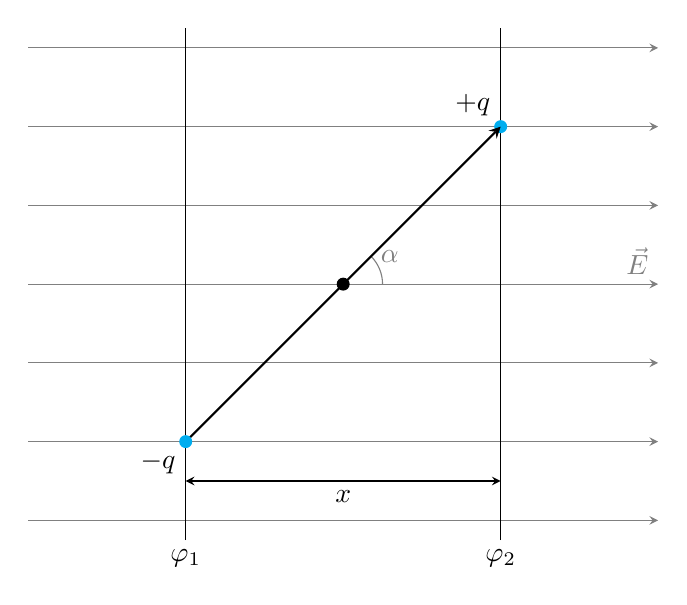
\begin{tikzpicture}[>=stealth]
	\foreach \y in {-3,-2,...,3}
		\draw[-latex, thin, gray, ->] (-4, \y) -- (4, \y);
	\node[gray, above left] at (4, 0) {$\vec{E}$};

	\draw[thin] (-2, -3.25) node[below] {$\varphi_1$} -- (-2, 3.25);
	\draw[thin] (2, -3.25) node[below] {$\varphi_2$} -- (2, 3.25);

	\draw[fill] (0, 0) circle [radius=0.075];

	\draw[gray] (0.5, 0) arc [radius=0.5, start angle=0, end angle=45] node[right] {$\alpha$};

	\draw[<->, thin] (-2, -2.5) -- (2, -2.5);
	\node[below] at (0, -2.5) {$x$};

	\draw[cyan, fill] (2, 2) circle [radius=0.075];
	\draw[thick, ->] (-2, -2) node[below left] {$-q$} -- (2, 2) node[above left] {$+q$};
	\draw[cyan, fill] (-2, -2) circle [radius=0.075];
\end{tikzpicture}
			\caption{Электрический диполь во внешнем постоянном электрическом поле}
		\end{figure}
		Полная потенциальная энергия\index{Энергия!диполя} диполя\index{Диполь!} во внешнем поле (рис.~\ref{fig:dipole3}):
			$$E_{\text{п}}=+q\varphi_2+(-q)\varphi_1=q(\varphi_2-\varphi_1)=-qEx=-qEl\cos{\alpha}=-Ed\cos{\alpha}.$$
		\begin{equation}
			E_{\text{п}}=-\vec{E}\cdot\vec{d}.
		\end{equation}
		Если диполь сонаправлен с~полем, то он обладает наименьшей энергией:
			$$\vec{d}\codirect\vec{E}, \quad E_{\text{п}}=-Ed.$$
		Таким образом, сонаправленное положение диполя с внешним полем~-- наиболее выгодное.

		\subsection{Электрическое поле диполя}

		\begin{figure}[h!]
			\label{fig:dipole4}
			\centering
			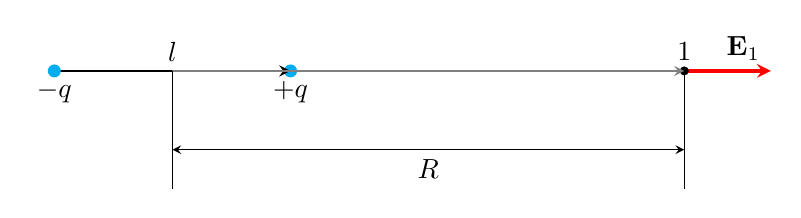
\begin{tikzpicture}[>=stealth]
	\draw[very thick, red, ->] (5, 0) -- (6.1, 0) node[black, above left] {$\textbf{E}_1$};
	\draw[cyan, fill] (0, 0) circle [radius=0.075];
	\draw[-latex, thick, ->] (-3, 0) node[below] {$-q$} -- (0, 0) node[below] {$+q$};
	\draw[cyan, fill] (-3, 0) circle [radius=0.075];
	\node[above] at (-1.5, 0) {$l$};

	\draw[fill] (5, 0) circle [radius=0.05];
	\draw[-latex, gray, semithick, ->] (-1.5, 0) -- (5, 0) node[black, above] {1};

	\draw[thin] (-1.5, 0) -- (-1.5, -1.5);
	\draw[thin] (5, 0) -- (5, -1.5);
	\draw[<->, thin] (-1.5, -1) -- (5, -1);
	\node[below] at (1.75, -1) {$R$};

\end{tikzpicture}

			\caption{Точка 1 на расстоянии $R$ от центра диполя}
		\end{figure}
		Найдем поле, создаваемое диполем в точках 1 и 2 на расстоянии $R$ от центра диполя, если $l\ll R$, где $l$ -- длина диполя (рис.~\ref{fig:dipole4}). Тогда
			$$E_1=k\frac{q}{(R-l/2)^2}-k\frac{q}{(R+l/2)^2}=\frac{kq\left[(R+l/2)^2-(R-l/2)^2\right]}{(R+l/2)^2(R-l/2)^2}=$$
			$$=\frac{2kqRl}{\left(R^2-(l/2)^2\right)^2}.$$
		Пренебрегая длиной диполя по сравнению с $R$, напишем
			$$E_1\simeq\frac{2kqRl}{R^4}=\frac{2kql}{R^3},$$
		\begin{equation}
			E_1\simeq\frac{2kd}{R^3}
		\end{equation}
		Поступим аналогично для точки 2:
		\begin{SCfigure}
			\documentclass{article}

\usepackage[latin1]{inputenc}
\usepackage{pgfplots}
\usepackage{tikz}
\usetikzlibrary{arrows}

\pgfplotsset{compat=1.10}

\begin{document}
\pagestyle{empty}

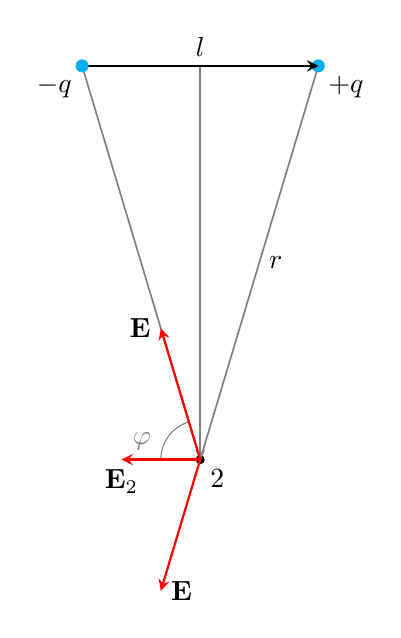
\begin{tikzpicture}[>=stealth]
	\draw[fill] (0, -5) circle [radius=0.05];
	\draw[gray, semithick, ->] (0, 0) -- (0, -5) node[black, below right] {2};
	\draw[gray, semithick] (0, -5) -- (-1.5, 0);
	\draw[gray, semithick] (0, -5) -- (1.5, 0);

	\draw[cyan, fill] (1.5, 0) circle [radius=0.075];
	\draw[-latex, thick, ->] (-1.5, 0) node[below left] {$-q$} -- (1.5, 0) node[below right] {$+q$};
	\draw[cyan, fill] (-1.5, 0) circle [radius=0.075];
	\node[above] at (0, 0) {$l$};
	\node[right] at (0.75, -2.5) {$r$};

	\draw[gray] ([shift=(106.6993:0.5cm)]0, -5) arc (106.6993:180:0.5cm) node[above left] {$\varphi$};

	\draw[red, thick, ->] (0, -5) -- (-0.5, -3.3334) node[black, left] {$\textbf{E}$};
	\draw[red, thick, ->] (0, -5) -- (-0.5, -6.6667) node[black, right] {$\textbf{E}$};
	\draw[red, thick, ->] (0, -5) -- (-1, -5) node[black, below] {$\textbf{E}_2$};
\end{tikzpicture}

\end{document}
			\caption{Точка 2 на расстоянии $R$ от центра диполя}
		\end{SCfigure}
			$$E_2=2E\cos{\varphi}=-2k\frac{q}{r^2}\cdot\frac{l/2}{r}=-\frac{kd}{r^3}=-\frac{kd}{\left(R^2+(l/2)^2\right)^{3/2}},$$
		\begin{equation}
			E_2\simeq-\frac{kd}{R^3}.
		\end{equation}
		Без доказательства приведем общую формулу:
		\begin{equation}
			\vec{E}=k\frac{3(\vec{d}\cdot\vec{n})\vec{n}-\vec{d}}{R^3} \quad \text{(верно при $l\ll R$)}.
		\end{equation}
		\begin{figure}[h!]
			\label{fig:dipole6}
			\centering
			\begin{tikzpicture}[>=stealth]
	\draw[cyan, fill] (1.5, 0) circle [radius=0.075];
	\draw[-latex, thick, ->] (-1.5, 0) node[below] {$-q$} -- (1.5, 0) node[below] {$+q$};
	\draw[cyan, fill] (-1.5, 0) circle [radius=0.075];
	\node[above] at (0, 0) {$\textbf{d}$};

	\node[above] at (2.5, -1.7) {$R$};

	\draw[thin, darkgray, ->] (0, 0) -- ++(-37:1cm) node[black, above] {$\textbf{n}$};
	\draw[thin, gray, ->]  (0, 0) -- ++(-37:5cm);

	\draw[red, very thick, ->] ++(-37:5cm) -- ++(-148:0.5cm) node[black, below] {$\textbf{E}$};
\end{tikzpicture}
			\caption{Поле диполя в точке на расстоянии $R$}
		\end{figure}
		Этой формулой описывается вся картина поля, создаваемого диполем. Заметим, что оно спадает как $\dfrac{1}{R^3}$.